\chapter{Software for Practical, Reproducible Analysis}

\section{Sparky extension}

Sparky \cite{sparky} is a popular program for interactive peak picking,
GSS construction, and chemical shift assignment and is available at
\url{http://www.cgl.ucsf.edu/home/sparky/}.  Sparky is implemented with
a core written in C++, and extensions in Python.  It is designed with 
extensibility as a key goal, and therefore has a convenient API through
which the core data model can be accessed from Python extensions.  The
extensions are also able to augment the user interface with additional
controls, as well as script common operations, and provide extra algorithms
for analysis.  Since Python is a full-featured programming language, 
it is also possible to interact with the filesystem, loading and dumping
data if necessary, as well as calling additional third-party tools.
% TODO add a picture of vanilla sparky

% TODO picture, explanation of Sparky data model
% TODO my extension in general terms.  data, approach, NMR-Star integration
% TODO my extension in implementation-specific terms.  
%   keyboard accelerator, etc.  

This Sparky extension is available online at 
\url{https://github.com/mattfenwick/SparkyExtensions}.  Installation is simple:
the extension file needs only to be placed in the appropriate directory
of an existing Sparky installation; see
\url{http://pine.nmrfam.wisc.edu/PINE-SPARKY/introduction.html}
for more information.  It is dual-licensed under the MIT and BSD licenses.

Sparky's familiarity, popularity, and extensibility make it an obvious choice
of platform for implementing reproducble data analysis approaches.  User
familiarity means that dialogs, menus, shortcuts, and data presentation are
identical, and therefore there is no learning curve outside of the new
reproducibility features.  Popularity means that many spectroscopists already
use Sparky, as evidenced by citations in the BMRB -- Sparky is cited
405 times in chemical shift assignments 
(\url{http://www.bmrb.wisc.edu/ftp/pub/bmrb/relational_tables/nmr-star3.1/Chem_shift_software.csv})
and 1813 times in general software use 
(\url{http://www.bmrb.wisc.edu/ftp/pub/bmrb/relational_tables/nmr-star3.1/Software.csv}).
An implicit advantage to the combination of extensibility with widespread 
familiarity and popularity is that new extensions can be added to a 
spectroscopist's analysis workflow without requiring a radical retooling of
the approach: the new extension can be used as much or as little as desired,
without causing the previous approach to necessarily be completely abandoned.
In my experience, this is a critical component of software adoption: the
ability to "play nice" with existing tools, by not creating a dichotomy
in software choice.
In summary, implementing a Sparky extension instead of creating a new analysis
tool from scratch greatly reduces the amount of software that must be written 
and maintained, allowing the focus to be kept on the real problem at hand,
which is reproducibility of analysis.


\section{NMR-Star library}
NMR-Star is the file format used by the BMRB \cite{bmrb} for archival of
NMR data.  As such data is useful for further studies, and archiving
data in the BMRB is the primary means of dissemination, it is important
to be able to work with NMR-Star files.

This library facilitates reproducibility by providing a robust interface
for working with NMR-Star files.  It allows both the creation of NMR-Star 
files as well as extraction of data -- for further querying -- of existing
files.  It is used by the previously mentioned Sparky extension.

To handle these files, a library was implemented both in Java 
\cite{fenwick2013} and in Python.  This library provides capabilities both
for reading and for writing NMR-Star files.  Although several tools for
dealing with NMR-Star files had already been implemented \cite{ccpn, bmrb},
there are several attributes of this library which set it apart:
\begin{itemize}
  \item error reporting of illegal input.  When malformed input is encountered,
    a useful, location-specific error is reported which includes sufficient
    information to quickly pinpoint and diagnose the problem.
  \item complete, standards-compliant NMR-Star syntax definition.
  \item open source under the MIT license.  This allows other interested 
    developers to peruse the source code to gain ideas, use the library in
    new applications, and modify and extend the library to fix problems or
    add new features if necessary.
  \item low coupling.  As a simple library, in order to use it, the library
    is simply imported using standard language facilities in order to use
    it through its programmatic API.  It does not require any external tools
    or dependencies, reducing the barrier to setup and installation.  It does
    not require learning to use additional tools or languages, merely the 
    host language; it takes advantage of the native facilities for abstraction
    and composition provided by the host language.
  \item high cohesion.  The library provides a simple, focused interface.
    This means it is easy to learn and use because it only deals with parsing
    the concrete syntax of NMR-Star files.
\end{itemize}
The library is freely available online (
\url{https://pypi.python.org/pypi/NMRPyStar}, 
\url{https://github.com/CONNJUR/StarParser}
).

An example of NMRPyStar in action is shown in Figure-\ref{nmrpystar_bmrb}.
As a regular Python library, in order to use it, it only needs to be 
imported into the client module.  Then, using a library for reading URLs
(which is bundled with Python distributions), an NMR-Star file is downloaded
from the BMRB \cite{bmrb}.  Then, it is parsed, and a parse tree, representing
the structure of the file, is returned; see Figure-\ref{nmrpystar_structure} 
Figure-\ref{nmrpystar_json}.  Finally, a query to extract the chemical shifts
from the parse tree is executed, and the results are used to calculate the
standard deviation of chemical shift assignments, grouped by residue type
and atom name; the results are in Figure-\ref{nmrpystar_query}.

The key to this example is the flexibility of the library: since it does not
impose any unnecessary restrictions on its use, it is easily adapted to
different situations; in this example, to reading NMR-Star files downloaded
programatically from the BMRB.  This flexibility is enabled by its bottom-up
design.  The parse tree, which is the output from the parser, holds a 
representation of the file, and queries are easily run against it.


\section{Connjur-ST}
The spectral reconstruction phase involves the processing of time-domain 
FID data to frequency-domain spectra.  There are several approaches for such
a transformation, including the Fourier Transform, Maximum Entropy reconstruction,
and Multi-dimensional decomposition \cite{nmrpipe, rnmrtk, mdd}.  There are
two key pieces to the data: the primary data (time-domain or frequency-domain),
which is typically in a binary format; and the meta data which records
important properties such as number of points, dwell time, and spectral width.

As covered earlier, spectral reconstruction involves the sequential application
of multiple functions, including linear prediction, zero fill, and apodization,
each of which must be parameterized appropriately, for the purposes of 
optimizing spectral characteristics such as peak shape, line width, and
signal-to-noise ratio.  In general, the exact effect of each of these operations
may depend on both the primary data as well as the meta data, and both types of
data may be modified as well.

Correct spectral reconstruction requires that the meta data is correctly 
handled, and reproducibility requires that all of the parameters are captured
as well (if the exact software versions used are captured, then it is not
necessary to capture the input and output primary and meta data from each
operation, since these can be regenerated as needed).  Two recent tools from
our lab, Connjur-ST \cite{connjur-st} and Connjur-WB, alleviate the
reproduciblity problem in the area of spectral reconstruction.

Connjur-ST, or Spectrum Translator, was designed with the general goal of
translating between various spectral formats, of which there are many, 
including Bruker, Varian/Agilent, XEasy, UCSF, RNMRTK, to name a few.  
It is necessary to convert between multiple formats during spectral 
reconstruction and analysis because different tools, each of which provides
valuable functionality, require different formats for input and output.
Thus, to use tools with differing format requirements, conversion will be
necessary.  While several tools do exist which implement specific conversions
between pairs of formats, there was previously no tool able to perform a
conversion between any two arbitrary formats.  The result was an artificial
restriction on combinations of tools, due to format constraints.  In addition,
attempting to remove this restriction by implementing additional tools is not
a satisfactory solution, because the number of tools required -- if each one
performs a single conversion -- grows with the square of the number of formats.
Such a solution clearly requires too much time and effort for initial
implementation, as well as future maintenance effort.

Spectrum Translator addresses this problem by means of a common data model,
which can be converted to and from any format.  For each format, a single
importer and a single exporter is required, which deal with conversion between
the format and Spectrum Translator's common data model.  This reduces the number
of converters required to the number of formats.  Thus, for translation between
any of five formats, the number of conversions required is reduced from 25 to
10 -- a 60\% reduction in the amount of conversions.  The discrepancy is even
greater when larger numbers of formats are considered.

This program is implemented in the Java programming language as an open source
library available from our website at \url{http://connjur.uchc.edu/downloads/st/}.
The advantage of using Java is that Java is "write once, run anywhere": Java
code, once compiled, may run on any Java Virtual Machine (JVM).  JVMs have been
implemented for many platforms, including Windows, Macintosh, and Linux.
This enables Spectrum Translator to run without modification on virtually any
computer.  A further advantage of Java is that as a popular programming 
language, there are many developers familiar with its syntax, semantics, 
class libraries, tooling, and deployment.

Spectrum Translator promotes data integration and consistency through the use
of a common data model and a single, unified conversion strategy.  It also
incorporates features for automatically reading meta data, which ease the
burden of meta data correctness for the user, which helps to ensure that the
meta data is more correct.  By applying a single interface to any format
conversion, the program has a smaller learning curve compared to learning
multiple differing interfaces for multiple tools.

Spectrum Translator has recently been extended to support non-uniform time-domain
data.  As the Rowland NMR Toolkit format is required in order to use its 
implementation of Maximum Entropy reconstruction \cite{rnmrtk}, Spectrum
Translator is an important enabler of the use of the technique, helping to 
make non-uniform data collection a realistic possibility for users who might
otherwise face significant hurdles in tooling.


\section{Connjur-WB}
Connjur-WB, or Workflow Builder, is a tool for spectral reconstruction which
builds on the successes of tools such as RNMRTK \cite{rnmrtk}, NMRPipe \cite{nmrpipe},
and Spectrum Translator \cite{connjur-st} by providing additional features
for data integration, reproducibility, meta data correctness, interactivity,
and expressiveness of spectral processing pipelines.  While Workflow Builder
is a standalone tool, it relies on external tools for the actual execution of
spectral processing functions.  This allows it to capitalize of user's 
familiarity with and knowledge of existing tools.

The general architecture of Workflow Builder is three tiers.  The first is 
the user-facing Graphical User Interface (GUI).  The GUI is responsible for
providing an intuitive, obvious, integrated, pleasant, and consistent experience
to users, and for ensuring that the critical information is present and easily
accessible.  This layer is implemented using Java's swing library.
At the other end is the third layer, or back-end, which is
responsible for data persistence, integrity, and integration.  The back-end
is implemented as a MySQL relational database management system (RDBMS), in
which are stored both the spectral meta data and the spectra themselves (if
desired); information specific to Workflow Builder and its internal model
of spectral reconstruction is also stored in the database.  The middle layer
is responsible for mediating the data exchanges between the GUI, the back-end,
and third-party tools such as RNMRTK and NMRPipe.

Workflow Builder allows viewing and modification of spectral meta data, which 
is important for ensuring correctness.  By capturing the meta data, Workflow
Builder facilitates reproducibility of spectral reconstruction.  Similar to
Spectrum Translator, Workflow Builder is implemented in Java, allowing it to
run anywhere that a JVM does; however, since it uses third-party tools which 
are platform-dependent, its usefulness on a platform is restricted if those
additional tools do not run there.  Workflow Builder also allows export of
spectral reconstruction data in XML and NMR-Star format.  The XML export
facilitates sharing between peers, while the NMR-Star exporting capabilities
enables reproducible archival as well.

A key component of Workflow Builder's success is its robust model of spectral
reconstruction, and the presentatio of its model to the user.  Workflow Builder
treats spectral reconstruction as a workflow composed of actors, which are
analagous to functions.  Each actor takes as input primary data and meta data,
and produces primary data and meta data as output.  The actor is responsible
for presenting the information required for correct parameterization of the
underlying function, and may contain significant logic and functionality.  A
notable example is the actor for Maximum Entropy reconstruction:  estimating
the noise correctly is a prerequisite for Maximum Entropy \cite{mobli2010non};
this actor is able to both estimate the noise level, as well as parameterize
the RNMRTK implementation \cite{rnmrtk}.  A portion of the model is shown
in Figure-\ref{wb_model}.

A further benefit of Workflow Builder's approach was noted at a workshop
hosted at the University of Connecticut Health Center in June, 2012.  For
beginning NMR spectroscopists, the barrier to entry is rather high.  Not only
is a large amount of domain knowledge required, but one must also be familiar
with the incidental complexity of NMR, including idiomatic expressions and
implicit data.  Workflow Builder was observed to greatly reduce the learning
curve due to its integration of necessary domain knowledge, explicit handling
of relevant data, and GUI-based presentation.  While such an interface may 
not be necessary for experts, beginners stand to gain from using such a 
tool.
% TODO add some screenshots


\section{Sample Scheduler}
The creation of effective sample schedules is an important aspect of efficient,
non-uniform data collection 
\cite{maciejewski2011random, rovnyak2004accelerated, mobli2010non}.  There
are multiple strategies for data collection.  The strategy used to generate
a sample schedule and the exact sample schedule used to collect time-domain
data has an effect on the quality of the data and on the ease of later 
analysis, due to properties such as artifacts (described by the point-spread
function), resolution, and sensitivity (related to signal-to-noise ratio).

A tool has been implemented to reproducibly capture the parameterizations
used in sample schedule creation, and is available online at
\url{https://github.com/mattfenwick/PyScheduler}.  The tool features a 
collection of popular algorithms for creating non-uniform sample schedules
with specific, desirable properties.  The algorithms are integrated within
a single uniform, consistent interface which allows all input parameters
and outputs to be captured and archived.  It integrates with previous work
done at UCHC \url{http://sbtools.uchc.edu/nmr/sample_scheduler/}.

The tool implements a data model of sample schedules; see 
Figure-\ref{schedule_model}.  The model deals with non-uniform quadrature
(partial component) \cite{maciejewski2011random}, non-uniform time delays, 
and non-uniform numbers of transients.  To my knowledge, the latter aspect of
non-uniform data collection remains a relatively unexplored domain, into
which this tool provides novel data representation capabilities.  In general,
an N-dimensional sample schedule, which is used for collecting (N+1)-dimensional
data sets, consists of a collection of N-dimensional pairs, each of which
has a time delay, represented as a positive integer, as well as a quadrature
phase, one of R or I.  Associated with each point is the number of transients
to collect, also modeled as a positive integer.  Within a sample schedule,
each N-dimensional pair represents a unique point in the space of the sample
schedule; for example, in a 2-dimensional schedule, the point (2,R),(4,I). 

One of the main strengths of this sample scheduler is its ability to flexibly
combine multiple different sampling approaches to create a schedule.  This
flexibility stems from its breakdown of sampling algorithms into independent
pieces with standard interfaces; by selecting one piece of each category, 
a combinatorial number of different choices can be made, resulting in sample
schedules with all imaginable kinds of properties.  This removes artificial
restrictions of what kinds of sample schedules can be constructed, making it
easier to experiment with various algorithsm.  The general categories of 
algorithms are:
\begin{itemize}
  \item coordinate generator.  Responsible for generating N-dimensional time
    delays.  Includes algorithms for generating all combinations within finite
    N-dimensional bounds, Poisson gap \cite{poissongap} sampling, as well
    as others.
  \item quadrature generator.  Responsible for generating the quadrature
    components.  Includes algorithms for full-component generation as well
    as various partial-component strategies.
  \item point selector.  Applies a filter to points based on coordinates,
    quadrature components, and number of transients, which can be used to create
    biased sampling schemes, such as exponentially-weighted decay
  \item point modifier.  Modifies some or all points in a sample schedule, 
    slightly changing the coordinates of points.  Includes algorithms for
    bursty \cite{maciejewski2009nonuniform} and blurred 
    \cite{hoch2008randomization} modifications.
  \item special point generator.  Forces the addition of specific points to
    a sample schedule, such as the first point along each axis.  Such properties
    are useful when evaluating the quality of spectra.
  \item formatter.  Includes facilities for generating textual output of a 
    sample schedule in RNMRTK \cite{rnmrtk}, Bruker, JSON, and Agilent formats.
\end{itemize}
Creating a sample schedule requires choosing from among the many algorithms 
available, and supplying the appropriate parameters.  While the various algorithms
are implemented as functions in standard Python modules, which could be imported
and used as a simple library, a command-line interface is also included.  The
interface requires the parameters -- both for choice of algorithm, as well as
for the algorithms themselves -- to be passed in through an appropriately
formatted file.  The parameters are then extracted and passed to the appropriate
algorithms, the sample schedule is constructed, and the output is returned. 

An example of the program in action is given in Figures \ref{schedule_parameters} 
and \ref{schedule_data}.  The first figure shows a parameter file in structured
text; this is passed in to the program.  The program then generates a sample
schedule, and writes the schedule out as a file, a part of which is shown in
the second figure.  Note that the parameter file includes parameters which 
apply to the schedule as a whole, as well as to specific dimensions; the output
file includes a single line for each set of time increments, and includes the
associated quadrature components.

% TODO point out features like decay, randomness
%   maybe this should include the text of the schedule, and the parameters too
This program was also integrated with an existing Java-based program written
by Mark Maciejewski, Val Gorbatyuk, and Jeffrey Hoch 
(\url{http://sbtools.uchc.edu/nmr/sample_scheduler/}), in order to leverage
the Java program's GUI capabilities for parameterizing sample schedule creation,
as well as displaying sample schedules and pointspread functions.  
Figure-\ref{sched1} shows a sample schedule created by my tool, by using the
Java GUI, which is then displayed in the Java GUI.  Note the increasing
sparsity as time delay increases in both non-uniformly sampled dimensions.
Figure-\ref{fft1} shows the pointspread function of this sample schedule,
indicating artifacts that it will create in the frequency domain.  This was 
calculated using a Fast Fourier Transform, and was also implemented in the
Java program by Maciejewski, Gorbatyuk and Hoch.  Figure-\ref{sched2} provides
a comparison to the first sample schedule; the parameterization is identical,
except that the first points along each axis are all collected (this is an
example of a special point selector).  This difference causes a noticable 
change in its pointspread function, seen in Figure-\ref{fft2}.

% TODO mention that it was used to generate data for the PNAS paper
% TODO add more discussion of the context, significance, and future value


\section{Discussion and conclusions}

% open source
All software discussed in this chapter is available under standard open source
licenses (either the MIT licence or the LGPL).  These licenses grant the rights
to inspect the source code, use the code in a program, modify the code, and
incorporate the code into a larger program.  While I do not believe that it is
necessary or desirable to force all scientists to publish source code under
open source licenses, I do believe that there are very real concrete benefits
to doing so.  

A major theme of this dissertation is reproducibility and its importance to
science.  Reproducibility is fostered by explicitness both in data collection
and analysis, as well as in communication between scientists, of results, 
protocols, and analyses.  Journal articles are an excellent means for 
communicating scientific findings, and the goal of such articles is typically
to include sufficient detail that the findings can be reproduced.  If the
article does not include sufficient detail, authors are often perfectly willing
to engage in communication with interested scientists to provide additional
detail.  However, in many cases, this does not apply to the software used to
produce a result.  Scientific software is often treated as proprietary 
intellectual property which may not be shared.  This leads to an interesting
constrast between the treatment of source code compared to data and experiemental
protocols.  If it were not for free and open communication of scientific results,
it is unlikely that science would have progressed as rapidly.  Similarly, by not
freely sharing source code, I believe that science's progress is restricted. 
While releasing code under open source licenses is clearly not the only way to
lift such restrictions, it seems to offer clear benefits to scientists and
funding agencies alike.

% reproducibility
The choice for which programs to describe in this section was driven by the
theme of reproducibility.  All of the programs covered here facilitate and 
support reproducible data analysis in a very real way.  The Sparky extension
provides functionality for tracking intermediate, derived, and extraneous data
during spectral analysis, and integrates with the NMR-Star library for recording
that data in NMR-Star files for later deposition to the BMRB, where the data is
made publicly available for dissemination.  Spectrum Translater, Workflow Builder
and the sample scheduler model and capture the meta data associated with 
data collection and spectral reconstruction, by making that meta data explicit,
visible, and modifiable.

% explicit data models
The use of explicit data models provides succinct, precise documentation as to
the intended use of a program and the semantics of its input and output data.
The design and dissemination of data models was an important part of the
implementation of the software programs described in this section.  A data 
model, expressed as an ER model or in some similar format, provides an
overview of the core functionality of a program through the data types 
which it documents.

% bottom-up design
A critical challenge that must be faced in the development of scientic software
is the apparent tradeoff between flexibility and adaptability on the one hand,
and robustness and strong guarantees on the other.  In the first case, the 
need is driven by the ever-changing nature of the scientific enterprise: as
new phenomena are discovered and studied, as new techniques and strategies for
analysis are invented and applied, the requirements of the supporting software
naturally must be correspondingly updated.  In the second case, scientists 
need to have at their disposal software which works correctly in order to 
guarantee accurate and reproducible computational analyses.  Much of the 
conviction that a software program works correctly comes from the experience 
of many users applying it; it is difficult to understand whether software 
works correctly without using it.  Over the course of my studies, I have 
explored an alternative approach to scientific software development which I 
believe can help address this issue by resolving the tradeoff.

This technique is known as "bottom-up" \cite{bottomup1994, bottomup2004} design
(as opposed to "top-down").  The core of this technique of software design is
to solve small problems simply and completely, and then to build bigger software
 -- whether programs or libraries -- by combining the small solutions.  The
opposing strategy of top-down design focuses on breaking problems down into 
smaller problems, and so on, until small enough problems are reached to be 
implemented directly as code.  While both strategies can lead to successful
outcomes, the key difference that has been observed is that while top-down
approaches typically require the solution to be known in advance and do not
react well to changing requirements, bottom-up solutions are easier to implement
effectively when the solution is not known in advance, and are also better
equipped for dealing with changing requirements 
\cite{topdown_bottomup, bottomup1994, bottomup2004}.  Therefore, it would seem
that bottom-up software is a more natural fit for science, due to the ever-changing
software needs of scientists.

Such has been my experience.  The tools presented here -- the NMR-Star library,
the sample scheduler, the Sparky extension, as well as Spectrum Translator and
Workflow Builder to a limited extent -- have been purposely designed with 
the bottom-up approach in mind.  The result is a library or tool that is 
extremely flexible, and readily adapted to different uses; extensions is also
straightforward.  The key realization encountered while designing these tools
was the importance of avoiding coupling \cite{coupling1992} whenever possible:
by specifying as few irrelevant details as possible, a software solution gains
flexibility to be applied in different ways as part of a large program.
 

% figures
\clearpage
\section{Figures}

\begin{figure}[h]
  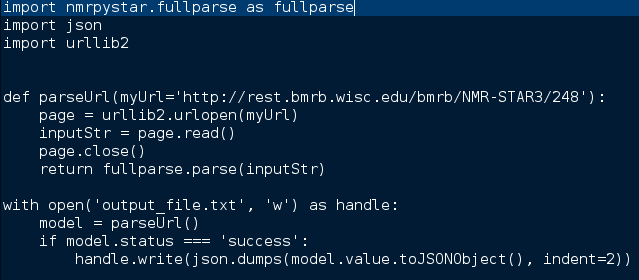
\includegraphics[scale=0.5]{figures/nmrpystar_bmrb}
  \caption[A code snippet of NMRPyStar]
          {A code snippet of NMRPyStar accessing the BMRB through its API.
           A file is downloaded, then parsed.}
  \label{nmrpystar_bmrb}
\end{figure}

\begin{figure}
  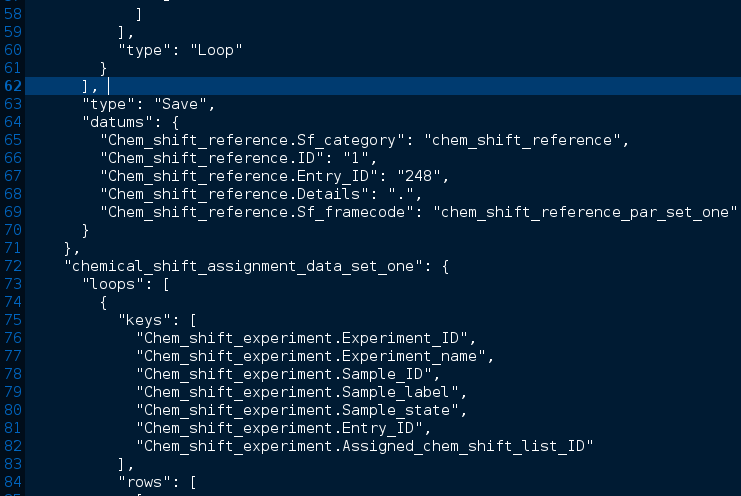
\includegraphics[scale=0.5]{figures/nmrpystar_json}
  \caption[NMRPyStar produces a parse tree as output]
          {NMRPyStar produces a parse tree as output, shown here in JSON format}
  \label{nmrpystar_json}
\end{figure}

\begin{figure}
  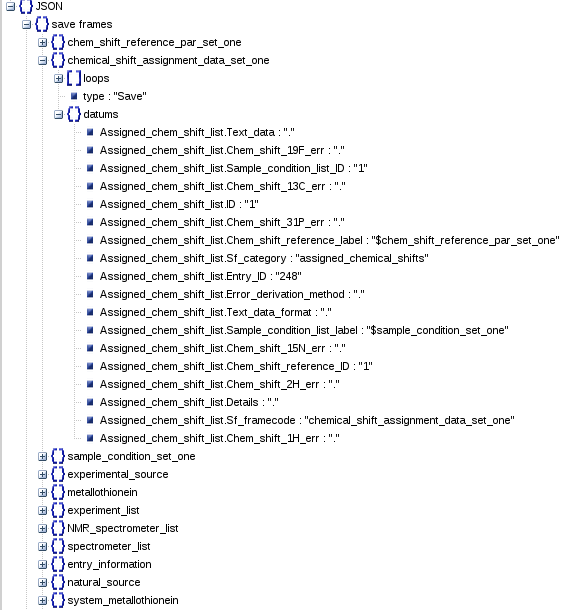
\includegraphics[scale=0.5]{figures/nmrpystar_structure}
  \caption{The parse tree can be used to extract key NMR information}
  \label{nmrpystar_structure}
\end{figure}

\begin{figure}
  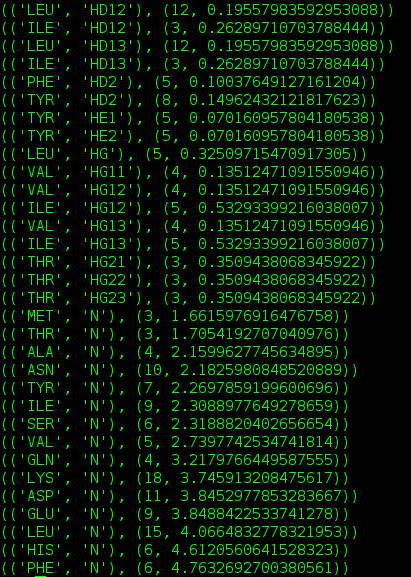
\includegraphics[scale=0.5]{figures/nmrpystar_query}
  \caption[The results of a query run against the parse tree]
          {The results of a query run against the parse tree.
           The query groups the assigned chemical shifts by
           amino acid type and atom name, and calculates the 
           standard deviation of each group.  The results are
           sorted by atom name.}
  \label{nmrpystar_query}
\end{figure}

\begin{figure}
  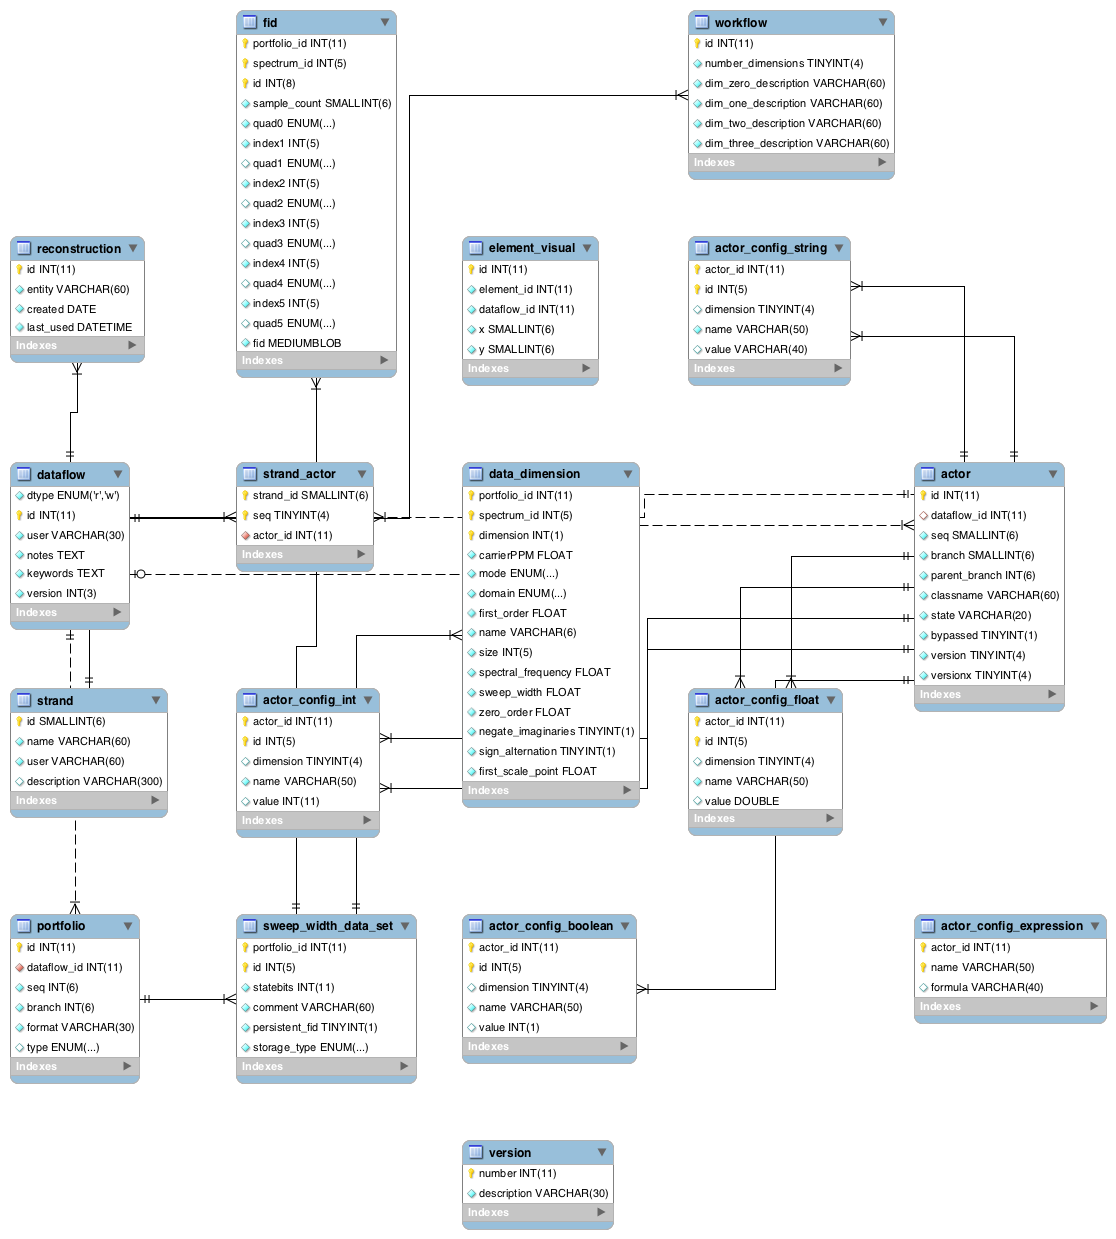
\includegraphics[scale=0.35]{figures/wb_model}
  \caption[Workflow Builder's data model]
          {Workflow Builder's data model.  Generated with MySQLWorkbench.}
  \label{wb_model}
\end{figure}

\begin{figure}
  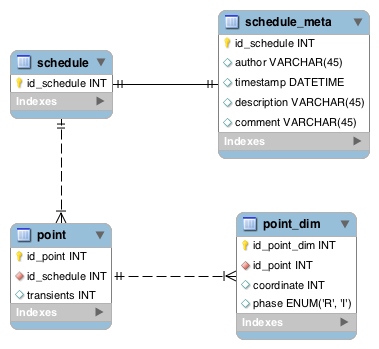
\includegraphics[scale=0.5]{figures/schedule_model}
  \caption[A data model of sample schedules]
          {A data model of sample schedules.  Created in MySQLWorkbench.}
  \label{schedule_model}
\end{figure}

\begin{figure}
  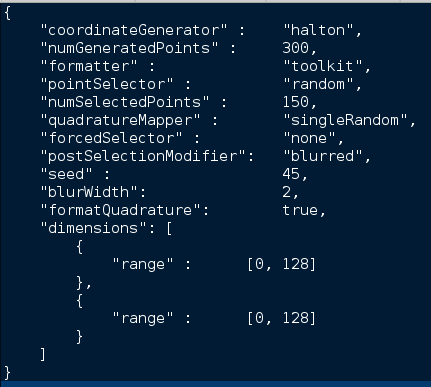
\includegraphics[scale=0.75]{figures/schedule_parameters}
  \caption{The parameter file input for a sample schedule.}
  \label{schedule_parameters}
\end{figure}

\begin{figure}
  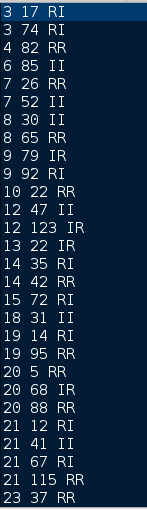
\includegraphics[scale=0.75]{figures/schedule_data}
  \caption{A sample schedule generated from the parameter file.}
  \label{schedule_data}
\end{figure}

\begin{figure}
  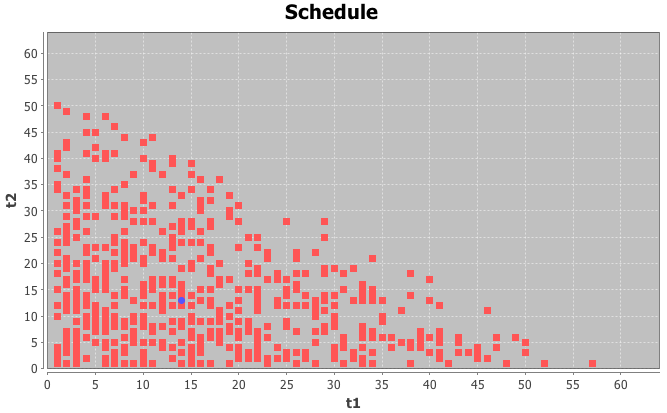
\includegraphics[scale=0.5]{figures/sched1}
  \caption{A graphical view of a sample schedule.}
  \label{sched1}
\end{figure}

\begin{figure}
  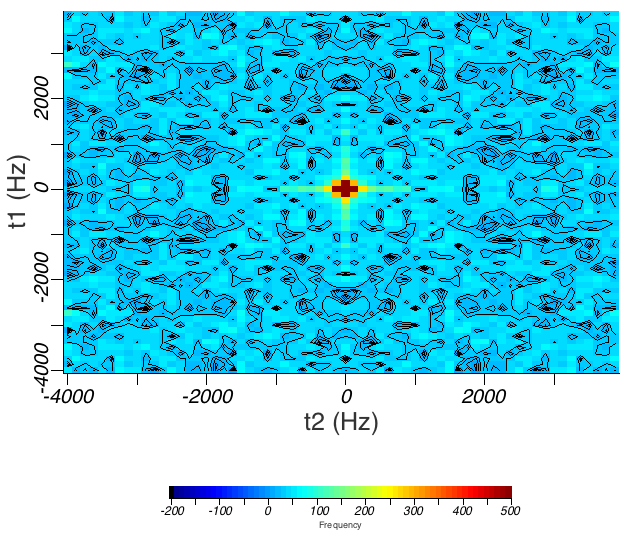
\includegraphics[scale=0.5]{figures/fft1}
  \caption{A sample schedule for which the first points along
           each axis are collected.}
  \label{fft1}
\end{figure}

\begin{figure}
  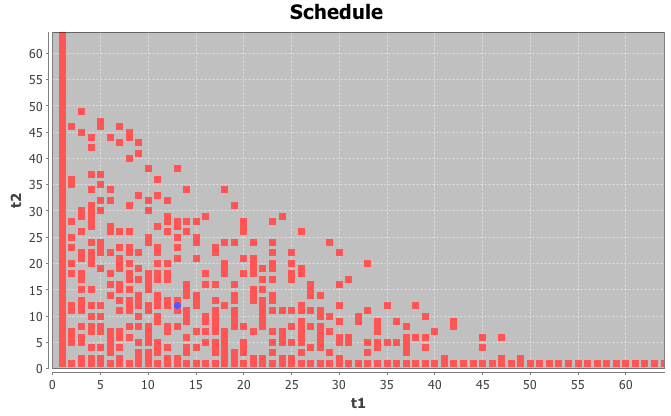
\includegraphics[scale=0.5]{figures/sched2}
  \caption{The pointspread function of the sample schedule, 
           calculated using a real-only FFT.}
  \label{sched2}
\end{figure}

\begin{figure}
  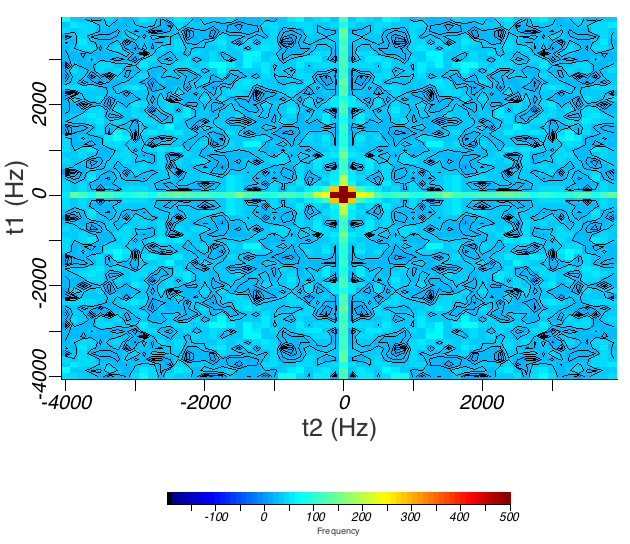
\includegraphics[scale=0.5]{figures/fft2}
  \caption{The pointspread function shows a noticable difference.}
  \label{fft2}
\end{figure}

